\documentclass[12pt, a4paper]{article}
%{{{
% Packages{{{
  \usepackage[hmarginratio=1:1,margin=1.2in]{geometry}
    \linespread{1.2}
  \usepackage{graphicx}
    \graphicspath{ {./images/} }
  \usepackage[dvipsnames]{xcolor}
  \usepackage[sc]{mathpazo}
  \usepackage{microtype}
  \usepackage{fancyhdr}
  \usepackage{titling}
    \renewcommand\maketitlehooka{\null\mbox{}\vfill}
    \renewcommand\maketitlehookd{\vfill\null}
  \usepackage{background}
  \backgroundsetup{contents=Swapnil, angle=0, opacity=1}

  \usepackage{listings}
    \lstset{
      frame=lrtb,
      language=Java,
      aboveskip=15px,
      belowskip=2px,
      showstringspaces=false,
      columns=flexible,
      basicstyle={\small\ttfamily},
      xleftmargin=5px,
      xrightmargin=5px,
      breakatwhitespace=true,
      tabsize=2
    }

  \usepackage{tcolorbox}
  \usepackage[utf8]{inputenc}
%}}}

% Footer section {{{
  % Creates footer
  \pagestyle{fancy}%
  \fancyhf{}%
  \lfoot{Assignment}
  \cfoot{\emph{Swapnil}}
  \rfoot{Page \thepage}
  \renewcommand{\headrulewidth}{0pt}% Line at the head invisible
  \renewcommand{\footrulewidth}{0.4pt}% Line at the footer visible
% }}}

% Title {{{
  \title{\Huge{\textsc{Practical on Programing in Java}}}
  \author{}
  \date{}
% }}}
%}}}

\begin{document}
\parindent0pt

%{{{
%Title page{{{
  \begin{titlingpage}
    \maketitle
    \thispagestyle{empty}
    %{{{
    \begin{tcolorbox}
      \textbf{\emph{Name}}: \verb+Swapnil Bhowmik+

      \textbf{\emph{Class Roll Number}}: \verb+7070+

      \textbf{\emph{University}}:

      \ \ \ \ \emph{Registration Number}: \verb+20200006768+

      \ \ \ \ \emph{Roll}: \verb+052120+

      \ \ \ \ \emph{Number}: \verb+400200086+

      \textbf{\emph{Paper Code}}: \verb+CACCC503L+
    \end{tcolorbox}
    %}}}
  \end{titlingpage}
  \newpage
%}}}

% ToC{{{
  \thispagestyle{empty}
  \tableofcontents
  \thispagestyle{empty}
  \vspace{2cm}
  \begin{tabular}{@{}p{2.4in}@{}}
  \hrulefill \\
    \textbf{Teacher's Signature}\\
  \end{tabular}
  \newpage
%}}}
%}}}

% Question 1{{{
\begin{tcolorbox}
\section{To find the sum of any number of integers entered as command line arguments}
\end{tcolorbox}
\subsection*{Date of Experiment:}
November 7\textsuperscript{th} 2022

\subsection*{Objective:}
\emph{\large{Write a program that reads command line arguments and compute the sum of the provided integers.}}

\subsection*{Compiler/Tools Used:}
\textbf{Development Kit}: \verb+jdk-7.0.5+

\textbf{Run-time Environment}: \verb+JavaSE-17+

\textbf{IDE:} \verb+eclipse 2022-09+

\subsection*{Program:}
\begin{lstlisting}
package assignment;

public class cmdArg {
  public static void main(String[] args) {
    int cnt, i = 0, n, s = 0;
    cnt = args.length;
    while (i < cnt) {
        n = Integer.parseInt(args[i]);
        s = s + n;
        i++;
    }
    System.out.println("The sum of integer is " + s);
  }
}
\end{lstlisting}
\newpage

\subsection*{Output:}
\begin{figure}[h]
  \centering
  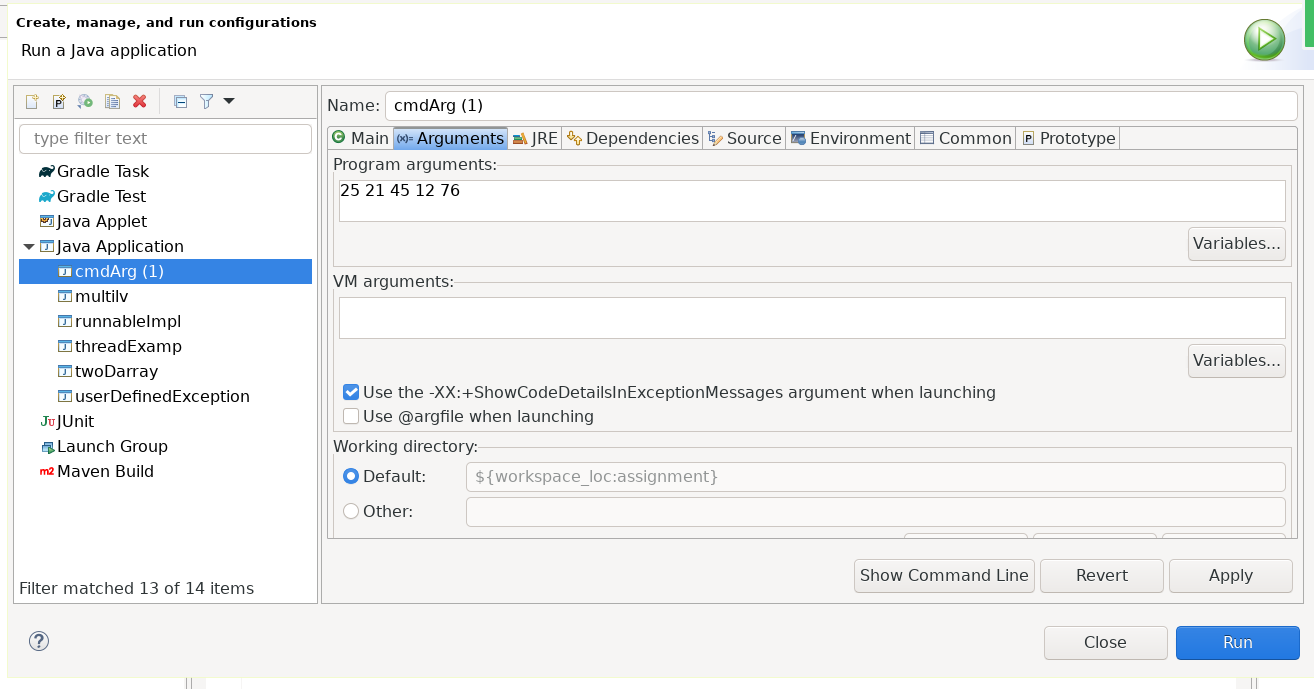
\includegraphics[width=\textwidth]{cmdarg1}
  \caption{Commandline Arguments}
\end{figure}
\begin{figure}[h]
  \centering
  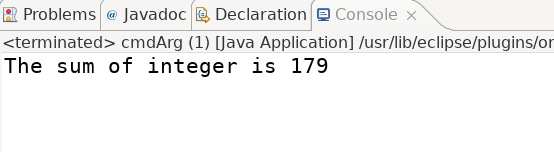
\includegraphics[width=\textwidth]{cmdarg2}
  \caption{Output}
\end{figure}
\newpage
%}}}

% Question 2{{{
\begin{tcolorbox}
\section{To find the factorial of a given number}
\end{tcolorbox}
\subsection*{Date of Experiment:}
November 7\textsuperscript{th} 2022

\subsection*{Objective:}
\emph{\large{Write a program that finds the factorial of a given number}}

\subsection*{Compiler/Tools Used:}
\textbf{Development Kit}: \verb+jdk-7.0.5+

\textbf{Run-time Environment}: \verb+JavaSE-17+

\textbf{IDE:} \verb+eclipse 2022-09+

\subsection*{Program:}
\begin{lstlisting}
package assignment;

import Java.util.Scanner;

public class FactNum {
  public static void main(String[] args) {
    Scanner sc = new Scanner(System.in);
    int a, fact = 1;
    System.out.println("Enter a number: ");
    a = sc.nextInt();

    System.out.println("Factorial is : " + facto(a));

  }
  public static int facto(int n) {
    if (n == 0) return 1;
    return n * facto(n - 1);
  }
}
\end{lstlisting}
\newpage

\subsection*{Output:}
\begin{figure}[h]
  \centering
  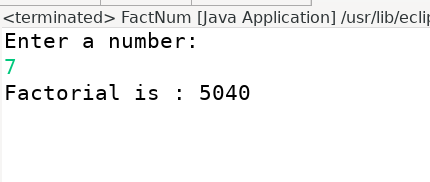
\includegraphics[width=\textwidth]{fact}
\end{figure}
\newpage
%}}}

% Question 3{{{
\begin{tcolorbox}
\section{To learn use of single dimensional array by defining the array dynamically.}
\end{tcolorbox}

\subsection*{Date of Experiment:}
November 7\textsuperscript{th} 2022
\subsection*{Objective:}
\emph{\large{Implement single dimensional array by defining the array dynamically}}

\subsection*{Compiler/Tools Used:}
\textbf{Development Kit}: \verb+jdk-7.0.5+

\textbf{Run-time Environment}: \verb+JavaSE-17+

\textbf{IDE:} \verb+eclipse 2022-09+

\subsection*{Program:}
\begin{lstlisting}
package assignment;
import Java.util.*;

public class oneDarray {
  public static void main(String[] args) {
    int a[], i, n;
    Scanner in = new Scanner(System.in);
    try {
      System.out.println("Enter how many number");
      n = in.nextInt();
      System.out.println("Enter array elements ");
      a = new int[n];

      for (i = 0; i < n; i++)
        a[i] = in.nextInt();
      System.out.println("The array elements are: ");

      for (i = 0; i < n; i++)
        System.out.print(a[i] + " ");
    } catch (Exception e) {}
  }
}
\end{lstlisting}

\subsection*{Output:}
\begin{figure}[h]
  \centering
  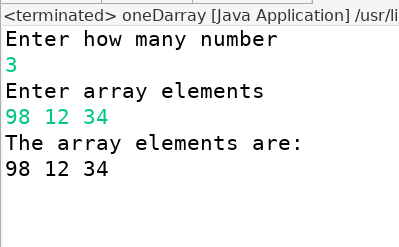
\includegraphics[width=\textwidth]{oneDarray}
\end{figure}
\newpage
%}}}

% Question 4{{{
\begin{tcolorbox}
\section{To learn use of lenth in case of a two dimensional array}
\end{tcolorbox}
\subsection*{Date of Experiment:}
November 10\textsuperscript{th} 2022

\subsection*{Objective:}
\emph{\large{Implement two dimensional array and learn the use of lenght}}

\subsection*{Compiler/Tools Used:}
\textbf{Development Kit}: \verb+jdk-7.0.5+

\textbf{Run-time Environment}: \verb+JavaSE-17+

\textbf{IDE:} \verb+eclipse 2022-09+

\subsection*{Program:}
\begin{lstlisting}
package assignment;
import Java.util.*;

public class twoDarray {
  public static void main(String[] args) {
    int a[][], r, c, i, j;
    Scanner in = new Scanner(System.in);
    try {
      System.out.println("Enter row and column for 2D array");
      r = in.nextInt();
      c = in.nextInt();
      System.out.println("Enter 2D elements");
      a = new int[r][c];
      for (i = 0; i < r; i++)
        for (j = 0; j < c; j++)
          a[i][j] = in.nextInt();
      System.out.println("2D elements are: ");
      for (i = 0; i < r; i++) {
        for (j = 0; j < c; j++)
          System.out.print(a[i][j] + " ");
        System.out.println();
      }
      System.out.println("The column lenght of 2D array is " + a.length);
      System.out.println("The row lenght of 2D array is " + a[0].length);
    } catch (Exception e) {}
  }
}
\end{lstlisting}

\subsection*{Output:}
\begin{figure}[h]
  \centering
  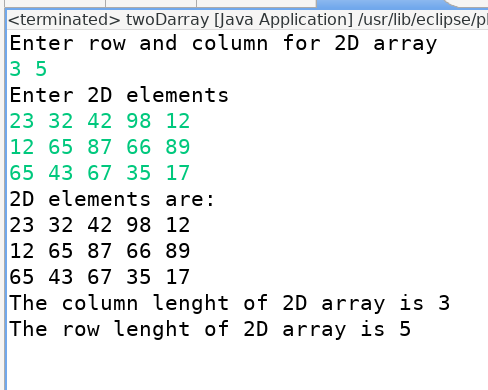
\includegraphics[width=\textwidth]{twoDarray}
\end{figure}
\newpage
%}}}

% Question 5{{{
\begin{tcolorbox}
\section{To convert a decimal to binary number}
\end{tcolorbox}
\subsection*{Date of Experiment:}
November 10\textsuperscript{th} 2022


\subsection*{Objective:}
\emph{\large{Convert decimal to binary}}

\subsection*{Compiler/Tools Used:}
\textbf{Development Kit}: \verb+jdk-7.0.5+

\textbf{Run-time Environment}: \verb+JavaSE-17+

\textbf{IDE:} \verb+eclipse 2022-09+

\subsection*{Program:}
\begin{lstlisting}
package assignment;
import Java.util.*;
public class dectobin {
  public static void main(String[] args) {
    int[] a;
      int r;
      Scanner in = new Scanner(System.in);
      System.out.println("Enter the value for n");
      int n = in.nextInt();
      a = new int[10];
      int i = 0;
      while (n > 0) {
        r = n % 2;
        a[i++] = r;
        n = n / 2;
      }
      for (int j = i - 1; j >= 0; j--)
        System.out.print(a[j]);
  }
}
\end{lstlisting}
\newpage

\subsection*{Output:}
\begin{figure}[h]
  \centering
  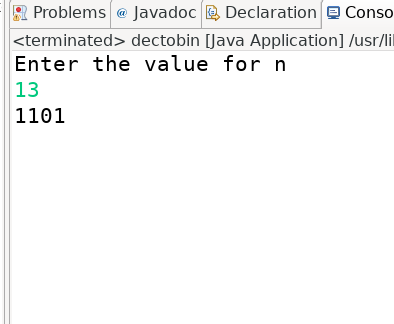
\includegraphics[width=\textwidth]{dectobin}
\end{figure}
\newpage
%}}}

% Question 6{{{
\begin{tcolorbox}
\section{To check if a number is prime or not, by taking the number as input from the keyboard}
\end{tcolorbox}
\subsection*{Date of Experiment:}
November 10\textsuperscript{th} 2022


\subsection*{Objective:}
\emph{\large{Check if a number is prime or not}}

\subsection*{Compiler/Tools Used:}
\textbf{Development Kit}: \verb+jdk-7.0.5+

\textbf{Run-time Environment}: \verb+JavaSE-17+

\textbf{IDE:} \verb+eclipse 2022-09+

\subsection*{Program:}
\begin{lstlisting}
package assignment;
import Java.util.*;

class prim {
  void check(int n) {
    int i;
    for (i = 2; i < n; i++) {
      if (n % i == 0) {
        System.out.println("Not prime");
        System.exit(0);
      }
    }
    System.out.println("Prime");
  }
}

public class primeno {
  public static void main(String[] args) {
    prim P = new prim();
    Scanner in = new Scanner(System.in);
    System.out.println("Enter any number :");
    int n = in.nextInt();
    P.check(n);
  }
}
\end{lstlisting}

\subsection*{Output:}
\setcounter{figure}{0}
\begin{figure}[h]
  \centering
  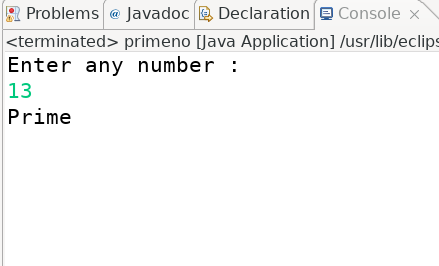
\includegraphics[width=0.7\textwidth]{prime}
  \caption{Case 1}
\end{figure}
\begin{figure}[h]
  \centering
  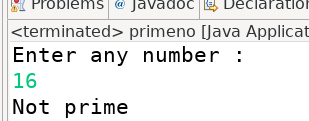
\includegraphics[width=0.7\textwidth]{notprime}
  \caption{Case 2}
\end{figure}
\newpage
%}}}

% Question 7{{{
\begin{tcolorbox}
\section{To find the sum of any number of integers interactively, i.e., entering every number from the keyboard, whereas the total number of integers is given as a command line argument}
\end{tcolorbox}

\subsection*{Date of Experiment:}
November 14\textsuperscript{th} 2022
\subsection*{Objective:}
\emph{\large{Find the sum of integers by taking input from the user via command line arguments}}

\subsection*{Compiler/Tools Used:}
\textbf{Development Kit}: \verb+jdk-7.0.5+

\textbf{Run-time Environment}: \verb+JavaSE-17+

\textbf{IDE:} \verb+eclipse 2022-09+

\subsection*{Program:}
\begin{lstlisting}
package assignment;
import Java.util.Scanner;

public class assignment7 {
  public static void main(String[] args) {
    int i;
    int s = 0;
    int n = Integer.parseInt(args[0]);
    int[] a;
    a = new int[n];
    System.out.println("enter the numbers one by one :");
    Scanner in = new Scanner(System.in);
    for (i = 0; i < n; i++) {
      a[i] = in.nextInt();
      s = s + a[i];
    }
    System.out.println("the sum of integer is " + s);
  }
}
\end{lstlisting}

\subsection*{Output:}
\setcounter{figure}{0}
\begin{figure}[h]
  \centering
  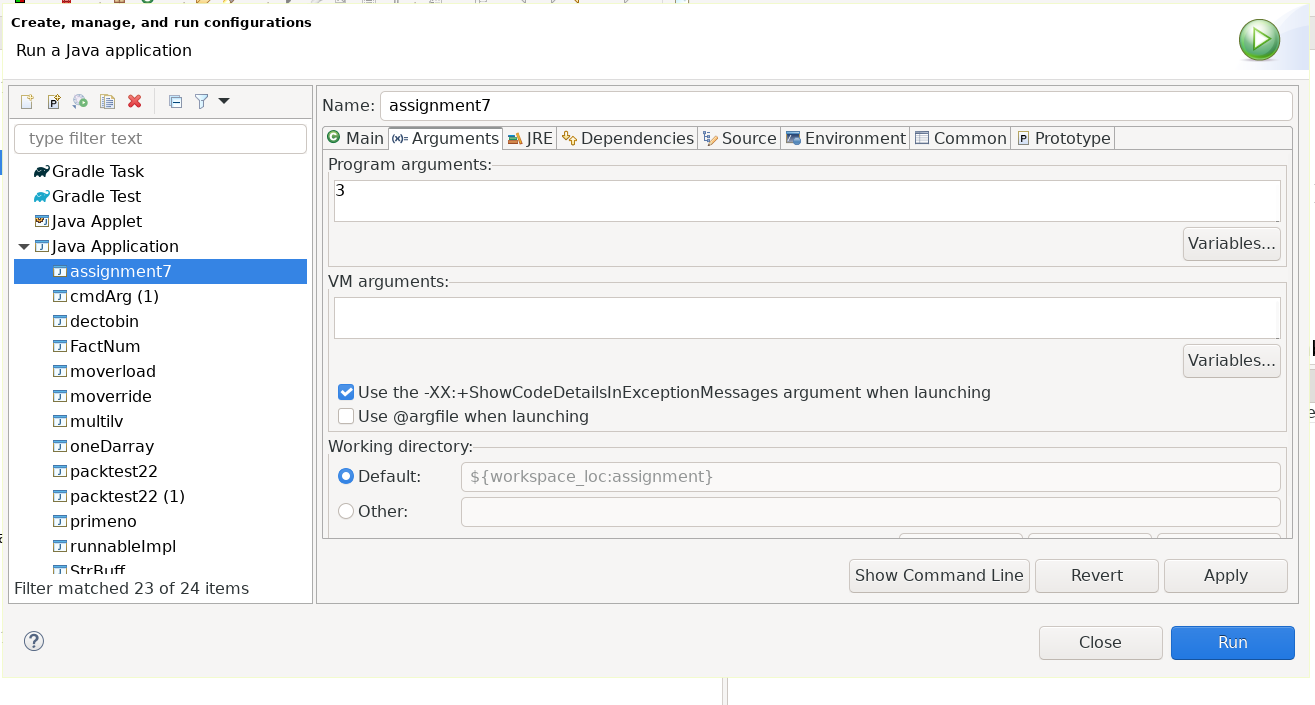
\includegraphics[width=\textwidth]{assign71}
  \caption{Commandline Arguments}
\end{figure}
\begin{figure}[h]
  \centering
  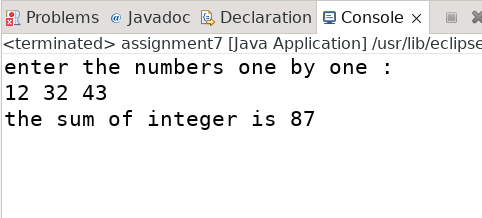
\includegraphics[width=\textwidth]{assign72}
  \caption{Output}
\end{figure}
\newpage
%}}}

% Question 8 {{{
\begin{tcolorbox}
\section{Write a Java Program to implement the concept of method overloading}
\end{tcolorbox}

\subsection*{Date of Experiment:}
November 14\textsuperscript{th} 2022
\subsection*{Objective:}
\emph{\large{Implement method overloading.}}

\subsection*{Compiler/Tools Used:}
\textbf{Development Kit}: \verb+jdk-7.0.5+

\textbf{Run-time Environment}: \verb+JavaSE-17+

\textbf{IDE:} \verb+eclipse 2022-09+

\subsection*{Program:}
\begin{lstlisting}
package assignment;

class Adder {
  int add(int a, int b) {
    return a + b;
  }
  int add(int a, int b, int c) {
    return a + b + c;
  }
}

public class moverload {
  public static void main(String[] args) {
    Adder A = new Adder();
    System.out.println(A.add(11, 11));
    System.out.println(A.add(22, 33, 44));
  }
}
\end{lstlisting}
\newpage

\subsection*{Output:}
\begin{figure}[h]
  \centering
  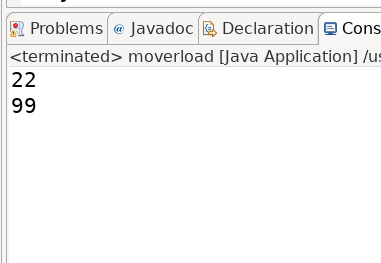
\includegraphics[width=\textwidth]{moverload}
\end{figure}
\newpage
%}}}

% Question 9 {{{
\begin{tcolorbox}
\section{Write a Java Program to implement the concept of method overriding.}
\end{tcolorbox}
\subsection*{Date of Experiment:}
November 14\textsuperscript{th} 2022

\subsection*{Objective:}
\emph{\large{Implement method overriding.}}

\subsection*{Compiler/Tools Used:}
\textbf{Development Kit}: \verb+jdk-7.0.5+

\textbf{Run-time Environment}: \verb+JavaSE-17+

\textbf{IDE:} \verb+eclipse 2022-09+

\subsection*{Program:}
\begin{lstlisting}
package assignment;

class Vehicle {
  void run() {
    System.out.println("Vehicle is running");
  }
}

class Bike extends Vehicle {
  //defining the same method as in the parent class  
  void run() {
    System.out.println("Bike is running safely");
  }
}

public class moverride extends Vehicle {
  public static void main(String[] args) {
    //Vehicle V=new Vehicle();
    Bike obj = new Bike();
    //calling the method with child class instance  
    obj.run();
    //V.run();
  }
}
\end{lstlisting}

\subsection*{Output:}
\begin{figure}[h]
  \centering
  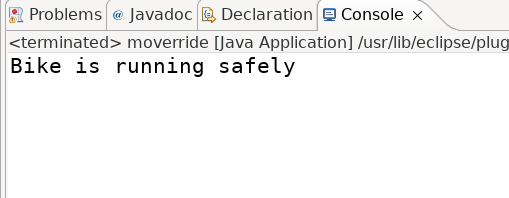
\includegraphics[width=\textwidth]{moverride}
\end{figure}
\newpage
%}}}

% Question 10 {{{
\begin{tcolorbox}
\section{Write a program that shows the working of different functions of Strings and StringBufferclass}{like \texttt{setCharAt()}, \texttt{setLength()}, \texttt{append()}, \texttt{insert()}, \texttt{concat()} and \texttt{equals()}. }
\end{tcolorbox}
\subsection*{Date of Experiment:}
November 25\textsuperscript{th} 2022

\subsection*{Objective:}
\emph{\large{Show the workings of different functions of Strings and StringBufferclass}}

\subsection*{Compiler/Tools Used:}
\textbf{Development Kit}: \verb+jdk-7.0.5+

\textbf{Run-time Environment}: \verb+JavaSE-17+

\textbf{IDE:} \verb+eclipse 2022-09+

\subsection*{Program:}
\begin{lstlisting}
package assignment;

public class StrBuff {
  public static void main(String[] args) {
    char[] ch = { 
      'j', 'a', 'v', 'a', 't', 'p', 'o', 'i', 'n', 't' 
    };

    String s = new String(ch);
    System.out.println("The string is " + s);
    System.out.println("the individyal first charecdter is " + ch[0]);
    String s1 = new String("Swapnil ");
    String s2 = new String("Bhowmik");
    s1.concat(s2);
    System.out.println("the string is " + s1.concat(s2));
    StringBuffer s3 = new StringBuffer("Swapnil ");
    StringBuffer s4 = new StringBuffer("Bhowmik");
    s3.append(s4);
    System.out.println("the string is " + s3);
    s3.insert(3, "Java ");
    System.out.println("the string is " + s3);
    s3.setLength(9);
    System.out.println("the string is " + s3);
    if (s1.equals(s2)) {
      System.out.println("the string are equal ...");
    } else {
      System.out.println("the string are not equal ...");
    }
    s4.setCharAt(3, 'x');
    System.out.println("the updated string is " + s4);
  }
}
\end{lstlisting}

\subsection*{Output:}
\begin{figure}[h]
  \centering
  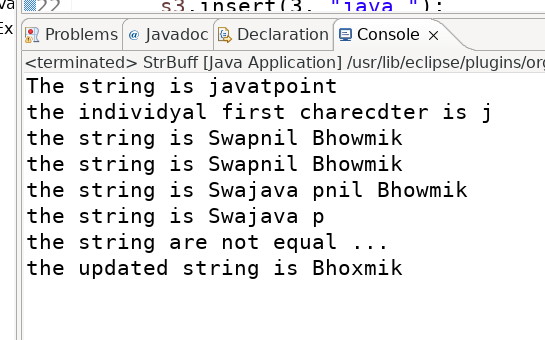
\includegraphics[width=\textwidth]{strbuff}
\end{figure}
\newpage
%}}}

% Question 11 {{{
\begin{tcolorbox}
\section{Write a Java program to demonstrate how packages are created and imported to another Java Program.}
\end{tcolorbox}

\subsection*{Date of Experiment:}
November 28\textsuperscript{th} 2022

\subsection*{Objective:}
\emph{\large{Demonstrate how packages are created and imported to another Java program}}

\subsection*{Compiler/Tools Used:}
\textbf{Development Kit}: \verb+jdk-7.0.5+

\textbf{Run-time Environment}: \verb+JavaSE-17+

\textbf{IDE:} \verb+eclipse 2022-09+

\subsection*{Program:}

\emph{\textbf{Package Create:::}}

\begin{lstlisting}
package empPack;
class test {
  public void disp_test() {
    System.out.println("Hello display test ");
  }
}
public class test1 extends test {
  public void disp_test1() {
    System.out.println("Hello display test 1");
  }
}
\end{lstlisting}

\emph{\textbf{Package import:::}}
\begin{lstlisting}
\underline
public class packtest22 {
  public static void main(String[] args) {
    test1 t = new test1();
    t.disp_test();
    t.disp_test1();
  }
}
\end{lstlisting}

\subsection*{Output:}
\begin{figure}[h]
  \centering
  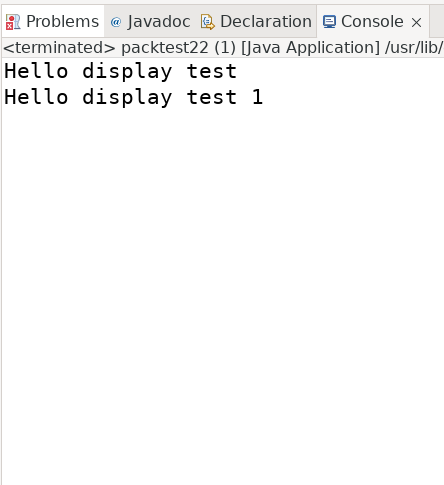
\includegraphics[width=\textwidth]{empPack}
\end{figure}
\newpage
%}}}

% Question 12 {{{
\begin{tcolorbox}
\section{Write a Java Program to implement the program of multiple inheritance through interface.}
\end{tcolorbox}

\subsection*{Date of Experiment:}
November 28\textsuperscript{th} 2022

\subsection*{Objective:}
\emph{\large{Implement single dimensional array by defining the array dynamically}}

\subsection*{Compiler/Tools Used:}
\textbf{Development Kit}: \verb+jdk-7.0.5+

\textbf{Run-time Environment}: \verb+JavaSE-17+

\textbf{IDE:} \verb+eclipse 2022-09+

\subsection*{Program:}
\begin{lstlisting}
package assignment;

interface I {
  final static int x = 13;
  public void disp_x();
}

class I_class {
  int x1;
  void get_x1() {
    x1 = 15;
  }
  void disp_x1() {
    System.out.println("The value of x1 is " + x1);
  }
}

class inter extends I_class implements I {
  public void disp_x() {
    System.out.println("The value of x is " + x);
  }
}

public class intrfceimpl {
  public static void main(String[] args) {
    inter i = new inter();
    i.disp_x();
    i.get_x1();
    i.disp_x1();
  }
}
\end{lstlisting}


\subsection*{Output:}
\begin{figure}[h]
  \centering
  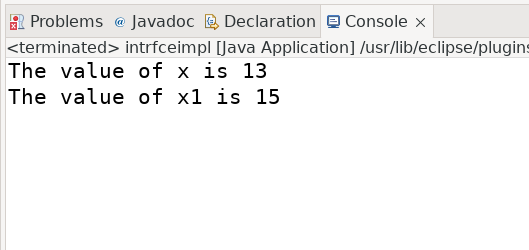
\includegraphics[width=\textwidth]{intrfceimpl}
\end{figure}
\newpage
%}}}

% Question 13 {{{
\begin{tcolorbox}
\section{Write a Java Program to implement multilevel inheritance.}
\end{tcolorbox}


\subsection*{Date of Experiment:}
November 28\textsuperscript{th} 2022

\subsection*{Objective:}
\emph{\large{Implement multilevel inheritance.}}

\subsection*{Compiler/Tools Used:}
\textbf{Development Kit}: \verb+jdk-7.0.5+

\textbf{Run-time Environment}: \verb+JavaSE-17+

\textbf{IDE:} \verb+eclipse 2022-09+

\subsection*{Program:}
\begin{lstlisting}
package assignment;

class A {
  void disp_A() {
    System.out.println("Display A");
  }
}
class B extends A {
  void disp_B() {
    System.out.println("Display B");
  }
}
class C extends B {
  void disp_C() {
    System.out.println("Display c");
  }
}
public class multilv {
  public static void main(String[] args) {
    C c = new C();
    c.disp_A();
    c.disp_B();
    c.disp_C();
  }
}
\end{lstlisting}

\subsection*{Output:}
\begin{figure}[h]
  \centering
  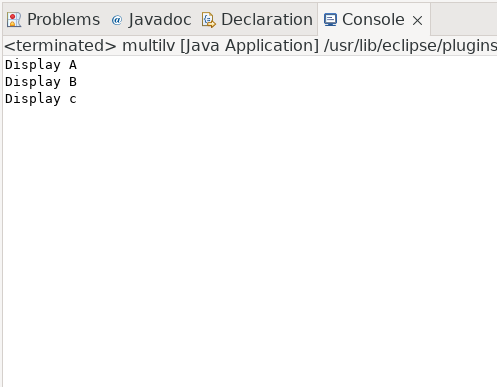
\includegraphics[width=\textwidth]{multilv}
\end{figure}
\newpage
%}}}

% Question 14 {{{
\begin{tcolorbox}
\section{Write a Java Program to demonstrate the exception handling using at-least three predefined exceptions.}
\end{tcolorbox}

\subsection*{Date of Experiment:}
December 1\textsuperscript{st} 2022

\subsection*{Objective:}
\emph{\large{Demonstrate exception handling using at-least three predefined exceptions.}}

\subsection*{Compiler/Tools Used:}
\textbf{Development Kit}: \verb+jdk-7.0.5+

\textbf{Run-time Environment}: \verb+JavaSE-17+

\textbf{IDE:} \verb+eclipse 2022-09+

\subsection*{Program:}
\begin{lstlisting}
package assignment;
import Java.util.*;
public class exceptionhandling {
  public static void main(String[] args) {
    Scanner in = new Scanner(System.in);
    try {
      int a[] = new int[5];
      String s = null;
      System.out.println(s.length());
    } catch (ArithmeticException e) {
      System.out.println("Arithmetic Exception occurs");
    } catch (ArrayIndexOutOfBoundsException e) {
      System.out.println("ArrayIndexOutOfBounds Exception occurs");
    } catch (NullPointerException e) {
        System.out.println("Null Pointer Exception");
    }
    System.out.println("rest of the code");
  }
}
\end{lstlisting}

\subsection*{Output:}
\begin{figure}[h]
  \centering
  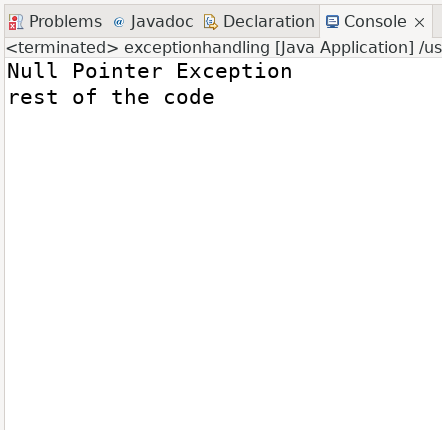
\includegraphics[width=\textwidth]{exceptionhandling}
\end{figure}
\newpage
%}}}

% Question 15 {{{
\begin{tcolorbox}
\section{Write a Java Program to demonstrate user defined exceptions.}
\end{tcolorbox}
\subsection*{Date of Experiment:}
December 1\textsuperscript{st} 2022

\subsection*{Objective:}
\emph{\large{Demonstrate user defined exceptions.}}

\subsection*{Compiler/Tools Used:}
\textbf{Development Kit}: \verb+jdk-7.0.5+

\textbf{Run-time Environment}: \verb+JavaSE-17+

\textbf{IDE:} \verb+eclipse 2022-09+

\subsection*{Program:}
\begin{lstlisting}
package assignment;

class InvalidAgeException extends Exception {
  public InvalidAgeException(String str) {
    super(str);
  }
}

public class userDefinedException {
  static void validate(int age) throws InvalidAgeException {
    if (age < 18) {
      throw new InvalidAgeException("age is not valid to vote");
    } else {
      System.out.println("welcome to vote");
    }
  }
  public static void main(String[] args) {
    try {
      validate(12);
    } catch (InvalidAgeException ex) {
      System.out.println("Caught the exception");

      System.out.println("Exception occured: " + ex);
      }
  }
}
\end{lstlisting}

\subsection*{Output:}
\begin{figure}[h]
  \centering
  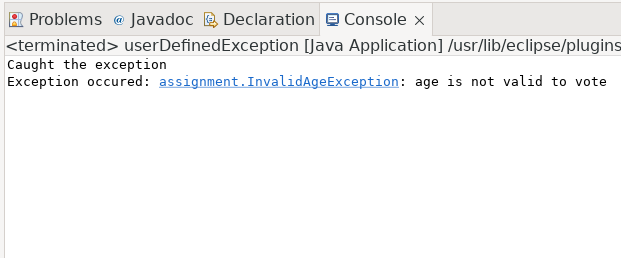
\includegraphics[width=\textwidth]{userDefinedException1}
\end{figure}
\newpage
%}}}

% Question 16 {{{
\begin{tcolorbox}
\section{Write a Java Program to demonstrate the concept of multi-threading.}
\end{tcolorbox}

\subsection*{Date of Experiment:}
December 2\textsuperscript{nd} 2022
\subsection*{Objective:}
\emph{\large{Demonstrate the concept of multi-threading.}}

\subsection*{Compiler/Tools Used:}
\textbf{Development Kit}: \verb+jdk-7.0.5+

\textbf{Run-time Environment}: \verb+JavaSE-17+

\textbf{IDE:} \verb+eclipse 2022-09+

\subsection*{Program:}
\begin{lstlisting}
package assignment;

class tA extends Thread {
  public void run() {
    for (int i = 1; i <= 5; i++)
      System.out.println("i = " + i);
  }
}

class tB extends Thread {
  public void run() {
    for (int j = 1; j <= 5; j++)
      System.out.println("j = " + j);
  }
}

class tC extends Thread {
  public void run() {
    for (int k = 1; k <= 5; k++)
      System.out.println("k = " + k);
  }
}

public class threadExamp {
  public static void main(String[] args) {
    tA A = new tA();
    tB B = new tB();
    tC C = new tC();
    A.start();
    B.start();
    C.start();
  }
}
\end{lstlisting}

\subsection*{Output:}
\begin{figure}[h]
  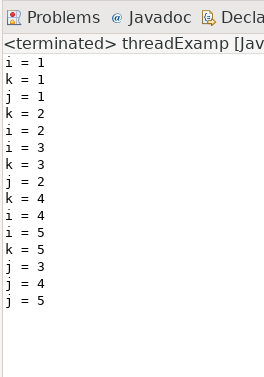
\includegraphics{threadExamp1}
\end{figure}
\newpage
%}}}

% Question 17 {{{
\begin{tcolorbox}
\section{Write a Java Program to demonstrate the concept of runnable interface.}
\end{tcolorbox}

\subsection*{Date of Experiment:}
December 2\textsuperscript{nd} 2022

\subsection*{Objective:}
\emph{\large{Demonstrate the concept of runnable interface.}}

\subsection*{Compiler/Tools Used:}
\textbf{Development Kit}: \verb+jdk-7.0.5+

\textbf{Run-time Environment}: \verb+JavaSE-17+

\textbf{IDE:} \verb+eclipse 2022-09+

\subsection*{Program:}
\begin{lstlisting}
package assignment;

class runnable1 implements Runnable {
	public void run() {
		System.out.println("Thread has ended");
	}
}

public class runnableImpl {
	public static void main(String[] args) {
		runnable1 r=new runnable1();
		Thread t=new Thread(r);
		t.start();
		System.out.println("Hi");
	}

}

\end{lstlisting}
\newpage

\subsection*{Output:}
\begin{figure}[h]
  \centering
  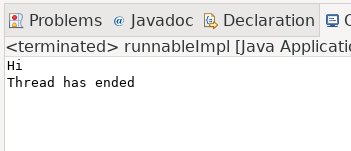
\includegraphics[width=\textwidth]{runnable}
\end{figure}
\newpage
%}}}

% Question 18 {{{
\begin{tcolorbox}
  \section{Write a Java program to demonstrate the insertion operation using JDBC}
\end{tcolorbox}
\subsection*{Date of Experiment:}
December 14\textsuperscript{th} 2022

\subsection*{Objective:}
\emph{\large{Demonstrate insertion operation using JDBC.}}

\subsection*{Compiler/Tools Used:}
\textbf{Development Kit}: \verb+jdk-7.0.5+

\textbf{Run-time Environment}: \verb+JavaSE-17+

\textbf{Database Server:} \verb+mysql+

\textbf{IDE:} \verb+eclipse 2022-09+

\subsection*{Program:}
\begin{lstlisting}
package jdbc_demo;

import Java.sql.*;
import Java.util.*;
public class insertJdbc {
  public static void main(String[] args) {
    try {
      Class.forName("com.mysql.cj.jdbc.Driver");
      Connection con = DriverManager.getConnection("jdbc:mysql://localho
        st:3306/jdbcdb", "root", "");

      Statement stmt = con.createStatement();
      Scanner dis = new Scanner(System.in);
      System.out.println("Enter Roll Number:");
      int s1 = dis.nextInt();
      System.out.println("Enter Student Name:");
      String s2 = dis.next();
      stmt.executeUpdate("insert into student values(" + s1 + ",'" + s2
        + "')");
      System.out.println("One Record Inserted in the table");
      con.close();
      System.out.println("Collection is closed.");
      } catch (ClassNotFoundException e) {} catch (SQLException e1) {
      System.out.println(e1);
    }
  }
}
\end{lstlisting}

\subsection*{Output:}
\begin{figure}[h]
  \centering
  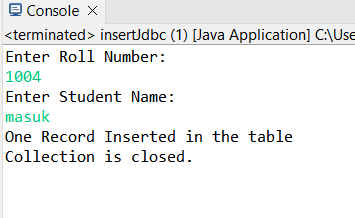
\includegraphics[width=\textwidth]{ijdbc}
\end{figure}
\newpage
%}}}

% Question 19 {{{
\begin{tcolorbox}
  \section{Write a Java program to demonstrate the view operation using JDBC}
\end{tcolorbox}
\subsection*{Date of Experiment:}
December 14\textsuperscript{th} 2022

\subsection*{Objective:}
\emph{\large{Demonstrate view operation using JDBC.}}

\subsection*{Compiler/Tools Used:}
\textbf{Development Kit}: \verb+jdk-7.0.5+

\textbf{Run-time Environment}: \verb+JavaSE-17+

\textbf{Database Server:} \verb+mysql+

\textbf{IDE:} \verb+eclipse 2022-09+

\subsection*{Program:}
\begin{lstlisting}
package jdbc_demo;
import Java.sql.*;
public class viewjdbc {
  public static void main(String[] args) {
    try {
      Class.forName("com.mysql.cj.jdbc.Driver");
      Connection con = DriverManager.getConnection("jdbc:mysql://localho
        st:3306/jdbcdb", "root", "");
      Statement stmt = con.createStatement();
      ResultSet rs = stmt.executeQuery("select * from student");
      while (rs.next()) {
        System.out.println(rs.getInt(1) + " " + rs.getString(2));
      }
    } catch (Exception e) {}
  }
}
\end{lstlisting}
\newpage

\subsection*{Output:}
\begin{figure}[h]
  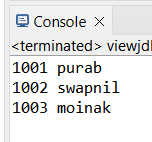
\includegraphics[width=0.5\textwidth]{vjdbc}
\end{figure}
\newpage
%}}}

% Question 20 {{{
\begin{tcolorbox}
  \section{Write a Java program to demonstrate the update operation using JDBC}
\end{tcolorbox}

\subsection*{Date of Experiment:}
December 14\textsuperscript{th} 2022

\subsection*{Objective:}
\emph{\large{Demonstrate update operation using JDBC.}}

\subsection*{Compiler/Tools Used:}
\textbf{Development Kit}: \verb+jdk-7.0.5+

\textbf{Run-time Environment}: \verb+JavaSE-17+

\textbf{Database Server:} \verb+mysql+

\textbf{IDE:} \verb+eclipse 2022-09+

\subsection*{Program:}
\begin{lstlisting}
package jdbc_demo;

import Java.sql.*;
import Java.util.*;
public class updatejdbc {
  public static void main(String[] args) {
    try {
      Class.forName("com.mysql.cj.jdbc.Driver");
      Connection con = DriverManager.getConnection("jdbc:mysql://localho
        st:3306/jdbcdb", "root", "");

      Statement stmt = con.createStatement();
      Scanner dis = new Scanner(System.in);
      System.out.println("Enter Roll Number to update name of student
        :");
      int s1 = dis.nextInt();
      System.out.println("Enter Student Name to be updated:");
      String s2 = dis.next();
      stmt.executeUpdate("update student set name=('" + s2 + "') where
        roll=(" + s1 + ")");
      System.out.println("Name updated successfully!!");
    } catch (ClassNotFoundException e) {} catch (SQLException e1) {
      System.out.println(e1);
    }
  }
}
\end{lstlisting}

\subsection*{Output:}
\begin{figure}[h]
  \centering
  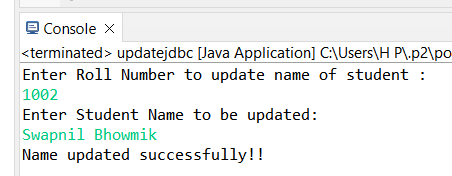
\includegraphics[width=\textwidth]{ujdbc}
\end{figure}
\newpage
%}}}

% Question 21 {{{
\begin{tcolorbox}
  \section{Write a Java program to demonstrate the delete operation using JDBC}
\end{tcolorbox}

\subsection*{Date of Experiment:}
December 14\textsuperscript{th} 2022

\subsection*{Objective:}
\emph{\large{Demonstrate delete operation using JDBC.}}

\subsection*{Compiler/Tools Used:}
\textbf{Development Kit}: \verb+jdk-7.0.5+

\textbf{Run-time Environment}: \verb+JavaSE-17+

\textbf{Database Server:} \verb+mysql+

\textbf{IDE:} \verb+eclipse 2022-09+

\subsection*{Program:}
\begin{lstlisting}
package jdbc_demo;

import Java.sql.Connection;
import Java.sql.DriverManager;
import Java.sql.SQLException;
import Java.sql.Statement;
import Java.util.Scanner;

public class deletejdbc {
  public static void main(String[] args) {
    try {
      Class.forName("com.mysql.cj.jdbc.Driver");
      Connection con = DriverManager.getConnection("jdbc:mysql://localho
        st:3306/jdbcdb", "root", "");

      Statement stmt = con.createStatement();
      Scanner dis = new Scanner(System.in);
      System.out.println("Enter Roll Number of student to be deleted:");
      int s1 = dis.nextInt();
      stmt.executeUpdate("delete from student where roll=(" + s1 + ")");
      System.out.println("One Record Deleted!!!");
      } catch (ClassNotFoundException e) {} catch (SQLException e1) {
          System.out.println(e1);
    }
  }
}
\end{lstlisting}

\subsection*{Output:}
\begin{figure}[h]
  \centering
  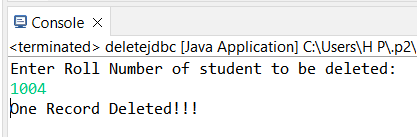
\includegraphics[width=\textwidth]{djdbc}
\end{figure}
\newpage
%}}}

% Question 22 {{{
\begin{tcolorbox}
  \section{Write a Java applet program to create a calculator and also perform addition, subtraction, multiplication and division operation.}
\end{tcolorbox}

\subsection*{Date of Experiment:}
January 7\textsuperscript{th} 2023

\subsection*{Objective:}
\emph{\large{To write a Java applet program that acts as a calculator and is about to perform various arithmatical operations.}}

\subsection*{Compiler/Tools Used:}
\textbf{Development Kit}: \verb+jdk-1.8+

\textbf{Run-time Environment}: \verb+JavaSE-17+

\textbf{IDE:} \verb+eclipse 2022-09+

\subsection*{Program:}
\begin{lstlisting}
package Subroto;
import java.awt.*;
import java.applet.*;
import java.awt.event.ActionEvent;
import java.awt.event.ActionListener;

public class calculator extends Applet implements ActionListener {
  TextField t1, t2;
  Label l1, l2, l3;
  Button b1, b2, b3, b4;
  int a, b, r;

  public void start() {
    t1 = new TextField(25);
    t2 = new TextField(25);
    l1 = new Label("Enter 1st number ");
    l2 = new Label("Enter 2nd number ");
    l3 = new Label("     ");
    b1 = new Button("ADD");
    b2 = new Button("SUBTRACT");
    b3 = new Button("PRODUCT");
    b4 = new Button("DIVISION");
    add(l1);
    add(t1);
    add(l2);
    add(t2);
    add(b1);
    add(b2);
    add(b3);
    add(b4);
    add(l3);
    b1.addActionListener(this);
    b2.addActionListener(this);
    b3.addActionListener(this);
    b4.addActionListener(this);
  }
  public void actionPerformed(ActionEvent ae) {
    String action = ae.getActionCommand();
    try {
      a = Integer.parseInt(t1.getText());
      b = Integer.parseInt(t2.getText());
    } catch (Exception e) {}
    if (action.equals("ADD")) {
      r = a + b;
    } else if (action.equals("SUBTRACT")) {
      r = a - b;
    } else if (action.equals("PRODUCT")) {
      r = a * b;
    } else if (action.equals("DIVISION")) {
      r = a / b;
    }
    l3.setText(String.valueOf(r));
  }
  public void paint(Graphics g) {
    g.setColor(Color.YELLOW);
  }
}
\end{lstlisting}

\pagebreak
\subsection*{Output:}
\begin{figure}[h]
  \centering
  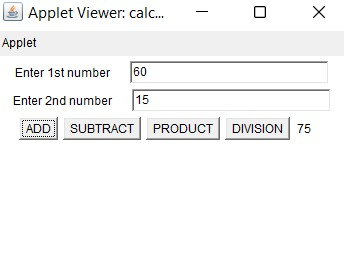
\includegraphics[width=0.7\textwidth]{calc}
\end{figure}
\pagebreak
%}}}

% Question 23 {{{
\begin{tcolorbox}
  \section{Write a Java program to demonstrate the delete operation using JDBC}
\end{tcolorbox}

\subsection*{Date of Experiment:}
January 7\textsuperscript{th} 2023

\subsection*{Objective:}
\emph{\large{Demonstrate delete operation using JDBC.}}

\subsection*{Compiler/Tools Used:}
\textbf{Development Kit}: \verb+jdk-1.8+

\textbf{Run-time Environment}: \verb+JavaSE-17+

\textbf{IDE:} \verb+eclipse 2022-09+

\subsection*{Program:}
\begin{lstlisting}
//package appletPrg;

import java.applet.*;
import java.awt.*;
import java.awt.event.*;
public class addMulApp extends Applet implements ActionListener {
  TextField t1 = new TextField(10);
  TextField t2 = new TextField(10);
  TextField t3 = new TextField(10);
  TextField t4 = new TextField(10);
  Label l1 = new Label("FIRST NO  :");
  Label l2 = new Label("SECOND NO :");
  Label l3 = new Label("SUM :");
  Button b = new Button("Calculate Sum and Product");
  Label l4 = new Label("Multiplication:");

  public void init() {

    add(l1);
    add(t1);
    add(l2);
    add(t2);
    add(b);
    add(l3);
    add(l4);
    add(t3);
    add(t4);

    b.addActionListener(this);

  }
  public void actionPerformed(ActionEvent e) {
    if (e.getSource() == b) {
      int n1 = Integer.parseInt(t1.getText());
      int n2 = Integer.parseInt(t2.getText());
      t3.setText(" " + (n1 + n2));
      t4.setText(" " + (n1 * n2));
    }
  }
}
\end{lstlisting}

\subsection*{Output:}
\begin{figure}[h]
  \centering
  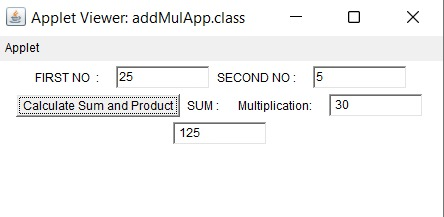
\includegraphics[width=0.7\textwidth]{addmul}
\end{figure}
\newpage
%}}}


\end{document}
